\documentclass{uc3mpracticas}

\usepackage{helvet}
\usepackage{multicol}
\renewcommand{\familydefault}{\sfdefault}
\usepackage{changepage}
\usepackage{geometry}
\usepackage{caption}
\usepackage{xcolor,colortbl}
\usepackage{makecell}

\definecolor{Gray}{gray}{0.85}
\definecolor{LightCyan}{rgb}{0.88,1,1}
\definecolor{LightGreen}{rgb}{0.29,1,0.39}

\newcolumntype{g}{>{\columncolor{Gray}}l}
\newcolumntype{b}{>{\columncolor{LightCyan}}c}


%%%%%%%%%%%%%%%%%%%%%%%%%%%%%%%%%%%%%%%%%%%%%%%%%%%%%%%%%%%%%%%%%%%%%%%%%%%%%%%%
%%%                   Plantilla Prácticas UC3M                               %%%
%%%                Universidad Carlos III de Madrid                          %%%
%%%                   Alejandro Valverde Mahou                               %%%
%%%%%%%%%%%%%%%%%%%%%%%%%%%%%%%%%%%%%%%%%%%%%%%%%%%%%%%%%%%%%%%%%%%%%%%%%%%%%%%%

%Permitir cabeceras y pie de páginas personalizados
\pagestyle{fancy}

%Path por defecto de las imágenes
\graphicspath{ {./images/} }

%Declarar formato de encabezado y pie de página de las páginas del documento
\fancypagestyle{doc}{
  %Cabecera
  \headerpr[1]{Problema de Clasificación: Parte II}{}{Redes de Neuronas Artificiales}
  %Pie de Página
  \footerpr{}{\textbf{UC3M}}{{\thepage} de \pageref{LastPage}}
}

%Declarar formato de encabezado y pie del título e indice
\fancypagestyle{titu}{%
  %Cabecera
  \headerpr{}{}{}
  %Pie de Página
  \footerpr{}{}{}
}


\appto\frontmatter{\pagestyle{titu}}
\appto\mainmatter{\pagestyle{doc}}


\begin{document}
  %Comienzo formato título
  \frontmatter


  %Portada 1 (Centrado todo)
  \centeredtitle{Images/LogoUC3M.png}{Grado en Ingeniería Informática}{Curso 2020/2021}{Redes de Neuronas Artificiales}{Problema de Clasificación: Parte II}{Clasificación de imágenes con Redes Convolucionales}

  \vspace{55mm}

  \authors{Alba Reinders Sánchez}{100383444}{Alejandro Valverde Mahou}{100383383}{}{}{}{}

  \newpage

  %Índice
  \tableofcontents

  \newpage

  %Comienzo formato documento general
  \mainmatter

\section{Introducción}

El problema consiste en clasificar imágenes donde las entradas de la red son directamente los píxeles de cada imagen. Se utiliza el conjunto de datos \textit{CIFAR10}, compuesto por \textbf{60000} imágenes en color (3 canales, \textit{RGB}) de \textbf{32x32} píxeles. El conjunto de datos se divide en 50000 imágenes para entrenamiento y 10000 para test.

\vspace{2mm}

Hay un total de \textbf{10 clases} con 6000 imágenes por clase, por lo que en este caso las clases sí están balanceadas, las diferentes clases son:

\begin{itemize}
  \begin{multicols}{5}
  \item 0 $\rightarrow$ \textit{airplane}
  \item 5 $\rightarrow$ \textit{dog}
  \item 1 $\rightarrow$ \textit{automobile}
  \item 6 $\rightarrow$ \textit{frog}
  \item 2 $\rightarrow$ \textit{bird}
  \item 7 $\rightarrow$ \textit{horse}
  \item 3 $\rightarrow$ \textit{cat}
  \item 8 $\rightarrow$ \textit{ship}
  \item 4 $\rightarrow$ \textit{deer}
  \item 9 $\rightarrow$ \textit{truck}
  \end{multicols}
\end{itemize}


El objetivo de la práctica es entrenar diferentes arquitecturas de \textbf{Perceptrón Multicapa} y \textbf{Redes de Neuronas Convolucionales} para analizar cómo influyen sus hiperparámetros en la resolución del problema de clasificación. Además de comparar sus resultados para comprobar cuál de las dos arquitecturas es más efectiva.



\section{Diseño, entrenamiento y evaluación del PM}

Inicialmente se intenta resolver este problema con el método de 'fuerza bruta'. Es decir, se aplana la información de los píxeles de las imágenes de entrada en un único vector y se entrena un \textbf{Perceptrón Multicapa} con estas entradas.

\vspace{2mm}

Para estudiar la eficacia de este acercamiento se realiza una pequeña experimentación probando distintas arquitecturas de red:

\begin{figure}[!h]
\begin{center}
  \begin{tabular}{|c|c|c|c|c|c|}
    \hline
    \rowcolor{Gray}
        \textbf{Arquitectura} & \textbf{\textit{epochs}}& \textbf{\textit{Accuracy} entrenamiento} & \textbf{\textit{Accuracy} test} & \textbf{\textit{Loss} entrenamiento} & \textbf{\textit{Loss} test}\\ \hline \hline
        (50)                  & 25                      &  0.5552                                  &  0.4743                         &  1.2606                              &  1.5040            \\ \hline
        (25)                  & 21                      &  0.5039                                  &  0.4493                         &  1.4128                              &  1.5678            \\ \hline
        (100)                 & 16                      &  0.5543                                  &  0.4922                         &  1.9684                              &  1.4483            \\ \hline
        (100,100)             & 30                      &  0.6442                                  &  0.5045                         &  0.9995                              &  1.4618            \\ \hline
        \rowcolor{LightGreen}
        (100, 100, 100)       & 23                      &  0.5900                                  &  0.5081                         &  1.1478                              &  1.4276            \\ \hline
  \end{tabular}
\end{center}
\caption*{Tabla Experimentos \textit{PM}}
\end{figure}

En cada uno de los experimentos se ajusta manualmente el número de \textit{epochs} óptimos para encontrar los mejores resultados posibles.

\vspace{2mm}

Se parte de la arquitectura dada en el tutorial y se prueba a modificar sus hiperparámetros a partir de ella. Primero se prueba a disminuir el número de neuronas, lo que no genera mejores resultados. Por tanto se prueba a aumentarlas y el \textit{accuracy} mejora, entonces se decide añadir una capa oculta más y también genera mejores resultados.

\vspace{1mm}

Como último experimento se configura una red con 3 capas ocultas de 100 neuronas cada una, este obtiene los mejores resultados. Sin embargo, el \textit{accuracy} en test que alcanza se queda estancado entorno a 0,5.

\vspace{2mm}

Tras esta experimentación se puede concluir que aumentar la complejidad de la arquitectura de la red, tanto en capas ocultas como en neuronas, hace que genere mejores resultados. Aunque no consigue superar un umbral, por lo que la utilización del \textit{PM} para resolver este problema no es del todo eficaz.

\vspace{3mm}

En las gráficas siguientes se puede ver la evolución de los valores de \textit{accuracy} y \textit{loss} de entrenamiento y test durante el aprendizaje de la red para el mejor experimento, que es el último de los realizados.

\newpage

\begin{figure}[!h]
\centering
\begin{minipage}{.52\textwidth}
  \centering
  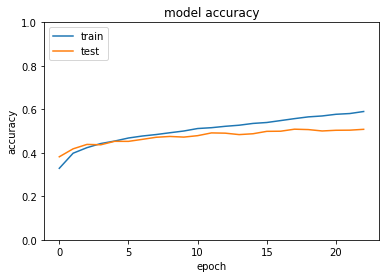
\includegraphics[width=.8\linewidth]{Images/accuracyPM.png}
  \caption*{\textit{Accuracy} en entrenamiento y test del \textit{PM}}
\end{minipage}%
\begin{minipage}{.52\textwidth}
  \centering
  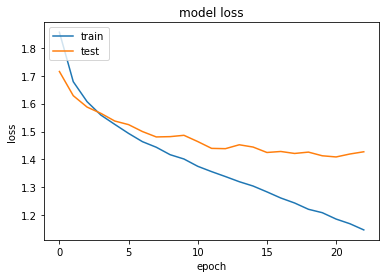
\includegraphics[width=.8\linewidth]{Images/lossPM.png}
  \caption*{\textit{Loss} en entrenamiento y test del \textit{PM}}
\end{minipage}
\end{figure}


A continuación se muestra la \textbf{matriz de confusión} resultante de este experimento. Además se añade el \textit{recall} para comprobar la precisión sobre cada una de las clases.

\begin{figure}[!h]
\begin{center}
  \begin{tabular}{|g|c|c|c|c|c|c|c|c|c|c|b|}
    \hline
    \rowcolor{Gray}
    Real \textbackslash Predicho  & \textbf{Airplane} & \textbf{Auto} & \textbf{Bird} & \textbf{Cat} & \textbf{Deer} & \textbf{Dog} & \textbf{Frog} & \textbf{Horse} & \textbf{Ship} & \textbf{Truck} & \textbf{\textit{Recall}}\\ \hline
            \textbf{Airplane} &  569 & 22 & 58 & 21 & 35 &  9 & 44 & 31 & 129 & 82 & 0.57 \\ \hline
            \textbf{Auto} & 41 & 516 & 15 & 25 & 14 &  7 & 45 & 21 & 84 & 232 & 0.52\\ \hline
            \textbf{Bird} & 86 & 10 & 334 & 83 & 142 & 55 & 177 & 64 & 29 & 20 & 0.33 \\ \hline
            \textbf{Cat} & 26 & 12 & 66 & 322 & 65 & 141 & 216 & 51 & 37 & 64  & 0.32\\ \hline
            \textbf{Deer} & 58 &  5 & 102 & 62 & 457 & 30 & 177 & 64 & 31 & 14  &0.46\\ \hline
            \textbf{Dog} &  21 & 11 & 80 & 211 & 60 & 321 & 145 & 85 & 34 & 32   & 0.32\\ \hline
            \textbf{Frog} & 10 &  4 & 32 & 53 & 86 & 27 & 733 & 18 & 13 & 24  & 0.73 \\ \hline
            \textbf{Horse} & 43 & 11 & 44 & 69 & 99 & 70 & 52 & 530 & 17 & 65 & 0.53 \\ \hline
            \textbf{Ship} & 91 & 44 &  8 & 16 & 20 & 10 & 28 & 18 & 675 & 90  & 0.68 \\ \hline
            \textbf{Truck} & 41 & 121 &  7 & 34 & 15 & 19 & 34 & 48 & 57 & 624  & 0.62 \\ \hline
      \end{tabular}
\end{center}
\caption*{Matriz de confusión mejor experimeto \textit{PM}}
\end{figure}

En esta matriz se puede apreciar que algunas clases como \textit{Frog} o \textit{Sheep} le resultan más fácil de clasificar al modelo. Mientras que otras clases como \textit{Bird}, \textit{Cat} o \textit{Dog} le resultan mucho más complicadas de diferenciar.







\section{Diseño, entrenamiento y evaluación de la CNN}

Una vez se ha experimentado con el \textit{PM} se intenta resolver este problema con una \textbf{Red Convolucional}. En este caso se aplican capas de convolución antes de aplanar la información.

\vspace{2mm}

Para estudiar la eficacia de esta aproximación se realiza la siguiente experimentación probando distintas arquitecturas. En cada uno de los experimentos, al igual que en el caso anterior, se ajusta manualmente el número de \textit{epochs} óptimos para encontrar los mejores resultados posibles.


\vspace{3mm}

\textit{Nota: la definición de la arquitectura sigue la siguiente terminología: $(n_1(k_1, Dd_1), n_2(k_2, Dd_2), ...)$ donde $n_i$ indica el número de filtros, $k_i$ el tamaño del kernel y $d_i$ el dropout}

\newpage

\begin{figure}[!h]
\begin{center}
  \begin{tabular}{|c|c|c|c|c|c|}
    \hline
    \rowcolor{Gray}
        \textbf{Arquitectura} & \textbf{\textit{epochs}}& \textbf{\textit{Accuracy} entrenamiento} & \textbf{\textit{Accuracy} test} & \textbf{\textit{Loss} entrenamiento} & \textbf{\textit{Loss} test}\\ \hline \hline
        (16(3))               & 20                      &  0.6960                                  &  0.6106                         &  0.8588                              &  1.1403            \\ \hline
        (16(3, D0.3))         & 47                      &  0.7127                                  &  0.6479                         &  0.8101                              &  1.0243            \\ \hline
        (32(3))               & 28                      &  0.7447                                  &  0.6121                         &  0.7041                              &  1.2311            \\ \hline
        (16(2))               & 14                      &  0.7007                                  &  0.6269                         &  0.8590                              &  1.1205            \\ \hline
        (16(2, D0.3))         & 7                       &  0.6558                                  &  0.6308                         &  0.9927                              &  1.0706            \\ \hline
        \makecell{(16(3, D0.3), \\ 16(3, D0.3))} & 20   &  0.7259                                  &  0.7006                         &  0.7813                              &  0.9050            \\ \hline
        \makecell{(16(3, D0.3), \\ 16(3, D0.3), \\ 16(3, D0.3))} & 44   &  0.7261                  &  0.6311                         &  0.7775                              &  1.0658            \\ \hline
        \makecell{(16(3, D0.5), \\ 16(3, D0.5))} & 43   &  0.7110                                  &  0.6401                         &  0.8234                              &  1.0642            \\ \hline
        \makecell{(16(3, D0.2), \\ 16(3, D0.2))} & 50   &  0.7640                                  &  0.7149                         &  0.6670                              &  0.8450            \\ \hline
        \makecell{(16(3, D0.1), \\ 16(3, D0.1))} & 13   &  0.7311                                  &  0.6952                         &  0.7690                              &  0.8952            \\ \hline
        \makecell{(16(4, D0.2), \\ 16(4, D0.2))} & 29   &  0.7716                                  &  0.7116                         &  0.6413                              &  0.8298            \\ \hline
        \rowcolor{LightGreen}
        \makecell{(16(5, D0.2), \\ 16(5, D0.2))}& 65   &  0.8179                                  &  0.7226                         &  0.5039                              &  0.8294            \\ \hline
        \makecell{(16(6, D0.2), \\ 16(6, D0.2))} & 31   &  0.7860                                  &  0.7107                         &  0.6018                              &  0.8393            \\ \hline
  \end{tabular}
\end{center}
\caption*{Tabla Experimentos \textit{CNN}}
\end{figure}


Se parte de la arquitectura dada en el tutorial y se prueba a modificar sus hiperparámetros a partir de ella. Tras probar esta configuración inicial se decide probar a añadir una capa de \textit{Dropout} de 0.3 para comprobar si mejoran los resultados, se puede ver que mejoran bastante.

\vspace{2mm}

Después se prueba a duplicar el número de filtros, pero esto no influye demasiado así que se puede decir que esto no es demasiado decisivo a la hora de mejorar los resultados. Por lo que se vuelven a establecer 16 filtros pero se prueba a disminuir el tamaño del kernel a 2. Esto tampoco parece influir en los resultados y por ello se prueba a añadir una capa de \textit{Dropout}, lo que produce una ligera mejora. Dado que cambiar los hiperparámetros de una única capa convolucional no hace que aumente el \textit{accuracy} en test, se decide añadir una segunda capa convolucional. Ambas con 16 filtros, tamaño de kernel 3 y \textit{Dropout} de 0.3, con esta arquitectura se consigue una mejora considerable.

\vspace{2mm}

Como aumentar el número de capas convolucionales ha dado buenos resultados, se prueba a añadir una tercera capa. Pero como esto hace que empeoren los resultados se decide seguir con la experimentación usando sólo dos capas convolucionales. Se puede concluir que aumentar demasiado la complejidad de la red hace que los resultados dejen de ser buenos.

\vspace{2mm}

A continuación se prueba a modificar el \textit{Dropout}, primero a aumentarlo. Como se ve que no mejora, se prueba a diminuirlo, obteniendo un mejor resultado con un \textit{Dropout} de 0.2. Tras esto se prueba a aumentar el tamaño del kernel

61

\begin{figure}[!h]
\begin{center}
  \begin{tabular}{|g|c|c|c|c|c|c|c|c|c|c|b|}
    \hline
    \rowcolor{Gray}
    Real \textbackslash  Predicho  & \textbf{Airplane} & \textbf{Auto} & \textbf{Bird} & \textbf{Cat} & \textbf{Deer} & \textbf{Dog} & \textbf{Frog} & \textbf{Horse} & \textbf{Ship} & \textbf{Truck} & \textbf{\textit{Recall}} \\ \hline
            \textbf{Airplane}  &      735  & 12 &  50 &  19 &  17 &  10 &  12 &  11 &  83 &  51 & 0.73 \\ \hline
            \textbf{Auto}   &      14 & 813 &   4 &   9 &   5 &   2 &   9 &   4 &  27 & 113 &  0.81  \\ \hline
            \textbf{Bird}  & 67 &  6 & 524 &  78 & 125 &  76 &  67 &  27 &  13 &  17 & 0.52 \\ \hline
            \textbf{Cat} &  26 &  8 & 50 & 556 & 81 & 151 & 62 & 22 & 26 & 18 & 0.56 \\ \hline
            \textbf{Deer} & 24 &  2 & 44 & 40 & 764 & 25 & 35 & 41 & 18 &  7 & 0.76\\ \hline
            \textbf{Dog}  & 16  & 7 & 35 & 193 & 55 & 603 &  22 &  51 &  8 & 10 & 0.60 \\ \hline
            \textbf{Frog} &  8 &  4 & 23 & 69 & 68 & 28 & 784 &  2 & 11 &  3 & 0.78\\ \hline
            \textbf{Horse} &  20 &  5 & 29 & 36 & 73 & 57 &  4 & 755 &  5 & 16 & 0.76 \\ \hline
            \textbf{Ship} & 44 & 22 & 13 & 13  & 6  & 3  & 6 &  4 & 849 & 40  & 0.85 \\ \hline
            \textbf{Truck} & 33 &  57 &  5 &  8 & 10 &  8 &  2 &  9 & 25 & 843 & 0.84\\ \hline
      \end{tabular}
\end{center}
\caption*{Matriz de confusión mejor experimeto \textit{CNN}}
\end{figure}

\section{Comparación PM y CNN}




\section{Conclusión}









\end{document}
